\chapter{Scatterplot And Correlation}

\section{Response Variable versus Explanatory Variable}
\textbf{Response/Dependent variable} measures an outcome of a study. 

\vspace{0.2cm}

\noindent \textbf{Explanatory/Predictor/Independent variable} may explain or influence changes in a response variable. 

\subsubsection*{Example 1}
How does drinking beer affect the level of alcohol in our blood? The legal limit for driving in all states is 0.08\%. Student volunteers at The Ohio State University drank different numbers of cans of beer. Thirty minutes later, a police officer measured their blood alcohol content. Consider \textit{number of cans of beer consumed} and \textit{blood alcohol level}, what is the predictor/explanatory variable and what is the response variable? 

\vspace{0.2cm}

\textbf{Solution}

\vspace{0.2cm}

\noindent Explanatory/Predictor variable: \textit{number of cans of beer consumed}

\noindent Response variable: \textit{blood alcohol level} 

\subsubsection*{Example 2}
The price of renting an apartment tends to increase when the apartment has more amenities. We want to examine this relationship between price and amenities. Consider \textit{price} and \textit{amenities}, what is the explanatory/predictor variable and what is the response variable? 

\vspace{0.2cm}

\textbf{Solution}

\vspace{0.2cm}

\noindent Explanatory/Predictor variable: \textit{amenities}

\noindent Response variable: \textit{price} 

\subsubsection*{Example 3}
In a study to determine whether surgery or chemotherapy results in higher survival rates for a certain type of cancer, whether or not the patient survived is one variable, and whether they received surgery or chemotherapy is the other. Consider \textit{survival rate} and \textit{treatment type}, what is the explanatory/predictor variable and what is the response variable?  

\vspace{0.2cm}

\textbf{Solution}

\vspace{0.2cm}

\noindent Explanatory/Predictor variable: \textit{treatment type}

\noindent Response variable: \textit{survival rate} 


\section{Scatterplot}
Scatterplot shows the relationship between two \textbf{quantitative} variables. Figure \ref{fig:scatterplot.jpg} is an example of a scatterplot.

\vspace{0.2cm}

\noindent \textbf{Note}: If there is an \textbf{explanatory/predictor} variable, it goes on the horizontal axis (x-axis); and the \textbf{response} variable goes on the vertical axis (y-axis). 

\begin{figure}[h!]
\centering
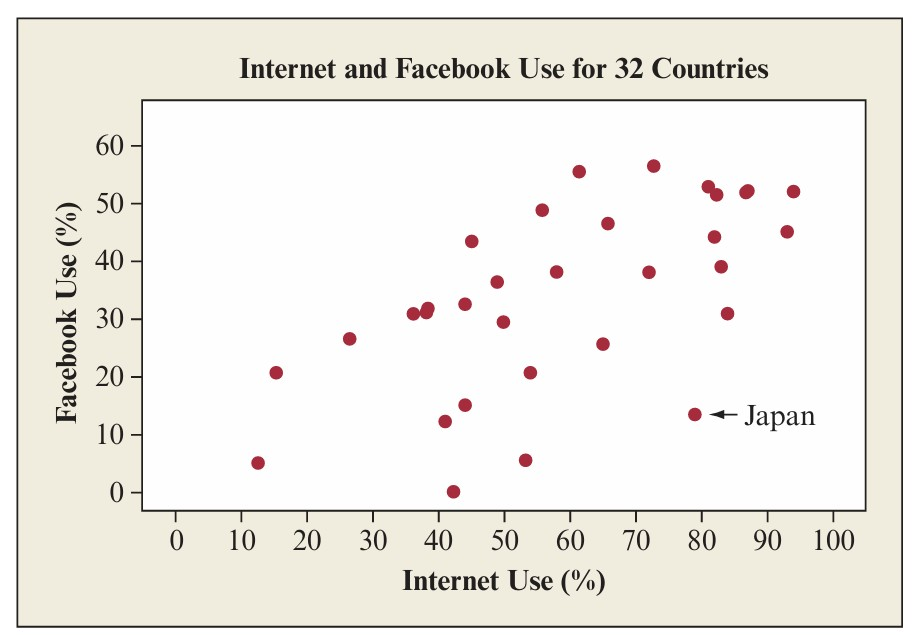
\includegraphics[width=0.6\textwidth]{figures/scatterplot.jpg}
\caption{Scatterplot for Internet and Facebook Use (in \% of the total population). The point for Japan is labeled and has coordinates \(x=79\%\) and \(y=13\%.\)}
\label{fig:scatterplot.jpg}
\end{figure}

\textbf{Note:} The standard deviation of the normal distribution is the distance from the center to the change-of-curvature points on either side.


\subsection{Positive Association versus Negative Association}
Two quantitative variables $x$ and $y$ are said to have a \textbf{positive} association when high values of $x$ tend to occur with high values of $y$, and when low values of $x$ tend to occur with low values of $y$. 

\vspace{0.2cm}
 
\noindent Two quantitative variables have a \textbf{negative} association when high values of one variable tend to pair with low values of the other variable, and low values of one pair with high values 
of the other. 

\vspace{0.2cm}

\noindent In simple terms:
 \begin{itemize}
    \item Positive association: as x increases, y tends increases. As x decreases, y tends decreases.
    \item Negative association: as x increases, y tends decreases. As x decreases, y tends increases. 
\end{itemize}

\subsubsection*{Example 1 about positive and negative associations}
It has been observed that between the ages of 0 to 16 years, the quantity of food eaten by people everyday increases with age. Is this relationship a negative or positive one? 

\vspace{0.2cm}

\textbf{Solution}

\vspace{0.2cm}

\noindent \textbf{Positive}. As age increases, the amount of food increases. 

\subsubsection*{Example 2 about positive and negative associations}
Jane needed to save money for her birthday. Her friend Joshua advised her to consider spending less money on gas by reducing the amount of distance she travels each week. Is the relationship between gas money and distance traveled negative or positive? 

\vspace{0.2cm}

\textbf{Solution}

\vspace{0.2cm}

\noindent \textbf{Positive}. The more distance you travel, the more money you spend on gas. And the less distance you travel, the less 
money you spend on gas. 

\subsubsection*{Example 3 about positive and negative associations}
Scientist have found that we are able to reduce our body fat by doing more body exercises or going to the gym a lot of times. The relationship between body fat and body exercises is negative or positive? 

\vspace{0.2cm}

\textbf{Solution}

\vspace{0.2cm}

\noindent \textbf{Negative}. As we do more body exercises, we are decreasing our body fat. 


\section{Correlation, $r$}
Correlation measures the \textbf{direction} and \textbf{strength} of the \textbf{linear} (straight-line) relationship between two \textbf{quantitative} variables. Correlation is usually denoted by $r$, it takes values between $-1$ and $+1$. Figure \ref{fig:scatterplot_B.jpg} shows examples of scatterplots and their values of $r$.
\begin{itemize}
    \item A positive value for $r$ indicates a positive association, and a negative value for $r$ indicates a negative association.
    \item The closer $r$ is to $\pm{1}$ the closer the data points fall to a straight line, and the stronger the linear association is. The closer $r$ is to $0$, the weaker the linear association is. 
    \item Even if the units of the variables change, the value of the correlation $r$ stays the same. 
\end{itemize}

\subsubsection*{Example 1 about Correlation}
Researchers asked mothers how much soda (in ounces) their kids drank in a typical day. They also asked these mothers to rate how aggressive their kids were on a scale of 1 to 10, with larger values corresponding to a greater degree of aggression. The correlation between amount of soda consumed and aggression rating was found to be $r = 0.3$. If the researchers had measured amount of soda consumed in liters instead of ounces, what would be the correlation? (There are 35 ounces in a liter.) 

\vspace{0.2cm}

\textbf{Solution}

\vspace{0.2cm}

\noindent The correlation would be \textbf{0.3}. Even if the units of the variables change, the value of the correlation $r$ stays the same.  

\begin{figure}[h!]
\centering
\includegraphics[width=1\textwidth]{figures/scatterplot_B.jpg}
\caption{Some Scatterplots and Their Correlations. The correlation gets closer to $\pm1$ when the data points fall closer to a straight line.}
\label{fig:scatterplot_B.jpg}
\end{figure}

\subsubsection*{Example 2 about Correlation}
A recent article in an educational research journal reports a correlation of $+0.8$ between math achievement and overall math aptitude. It also reports a correlation of $-0.8$ between math achievement and math anxiety. Which of the following interpretations is the most correct? 

a. The correlation of $+0.8$ is just as strong as the correlation of $-0.8$.  

b. It is impossible to tell which correlation is stronger. 

c. The correlation of $+0.8$ indicates a stronger relationship than the correlation of $-0.8$.  

\vspace{0.2cm}

\textbf{Solution}

\vspace{0.2cm}

\noindent \textbf{a. The correlation of $+0.8$ is just as strong as the correlation of $-0.8$.} 



